\documentclass[sigconf]{acmart}
\usepackage{amsmath}
\usepackage{tikz}
\usetikzlibrary{shapes,decorations,arrows,calc,arrows.meta,fit,positioning}

\begin{document}

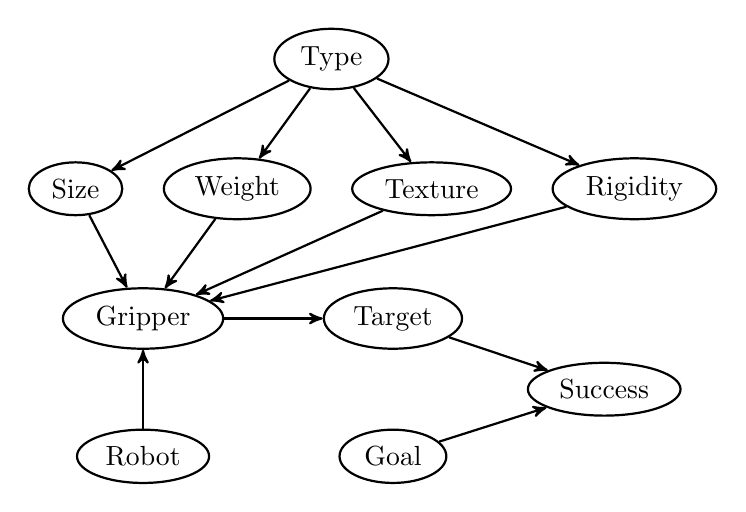
\begin{tikzpicture}[->,>=stealth',auto,node distance=0.5cm,
  thick,state/.style={ellipse,draw}]
\node [state] (Wg) {Weight};
\node [state, left = of Wg] (Sz) {Size};
\node [state, right = of Wg] (Tx) {Texture}; 
\node [state, right = of Tx] (Rd) {Rigidity}; 
\node [state, above = 1.25cm of $(Tx.west)!0.5!(Wg.east)$] (Ty) {Type};
\node [state, below = 1.25cm of $(Wg.west)!0.5!(Sz.east)$] (Gr) {Gripper};
\node [state, right = 1.25cm of Gr] (Ta) {Target};
\node [state, below = 1cm of Gr] (Ro) {Robot};
\node [state, below= 1cm of Ta] (Go) {Goal};
\node [state, right = 1.7cm of $(Ta.south)!0.5!(Go.north)$] (Sc) {Success};
\path[every node/.style={font=\sffamily\small}]
    (Ty) edge node [below] {} (Sz)
    (Ty) edge node [below] {} (Wg)
    (Ty) edge node [below] {} (Tx)
    (Ty) edge node [below] {} (Rd)
    (Sz) edge node [below] {} (Gr)
    (Wg) edge node [below] {} (Gr)
    (Tx) edge node [below] {} (Gr)
    (Rd) edge node [below] {} (Gr)
    (Gr) edge node [right] {} (Ta)
    (Ro) edge node [above] {} (Gr)
    (Ta) edge node [right] {} (Sc)
    (Go) edge node [right] {} (Sc);
\end{tikzpicture}

\end{document}